\chapter{Introduction}\label{ch:intro}

\section{Motivation}

When designing any system or application, there is how we theorise it will behave, and there is actually how it behaves. It is not uncommon to deploy a new application to production, only to find that it does not perform how we expected. However, diagnosing the performance issue typically cannot be resolved by simply inspecting the source code, looking for clues that may explain the unsatisfactory performance, but rather through measurement.

For example, if a web server takes significantly longer, compared to others, to resolve a particular kind of request, we need to understand which code-paths are being executed, and where in the system are unexpected amounts of time are being spent. Maybe the issue turns out to be that the CPU is stalled on memory I/O, or is spending too much time waiting for disk I/O. It could even be that the TCP connection between the client and the web server is sending too many TCP retransmits. The point is, without the ability to profile our systems or applications, we quickly become blind to the root cause of the performance issues we experience.

\subsection{Application to seL4}

seL4 is a microkernel, designed for building safety- and security-critical systems, due to its comprehensive formal verification and high performance \cite{SiteAboutSeL4}. It has proven to be sought-after in embedded systems, in cases which require a high degree of security or reliability. A core tenant of microkernels is to reduce the Trusted Computing Base (TCB). In seL4 this is achieved by hoisting OS functionality, that traditionally lives in the kernel, up into usermode servers, illustrated in Figure \ref{fig:sel4_microkernel}.

\begin{figure}[h!]
    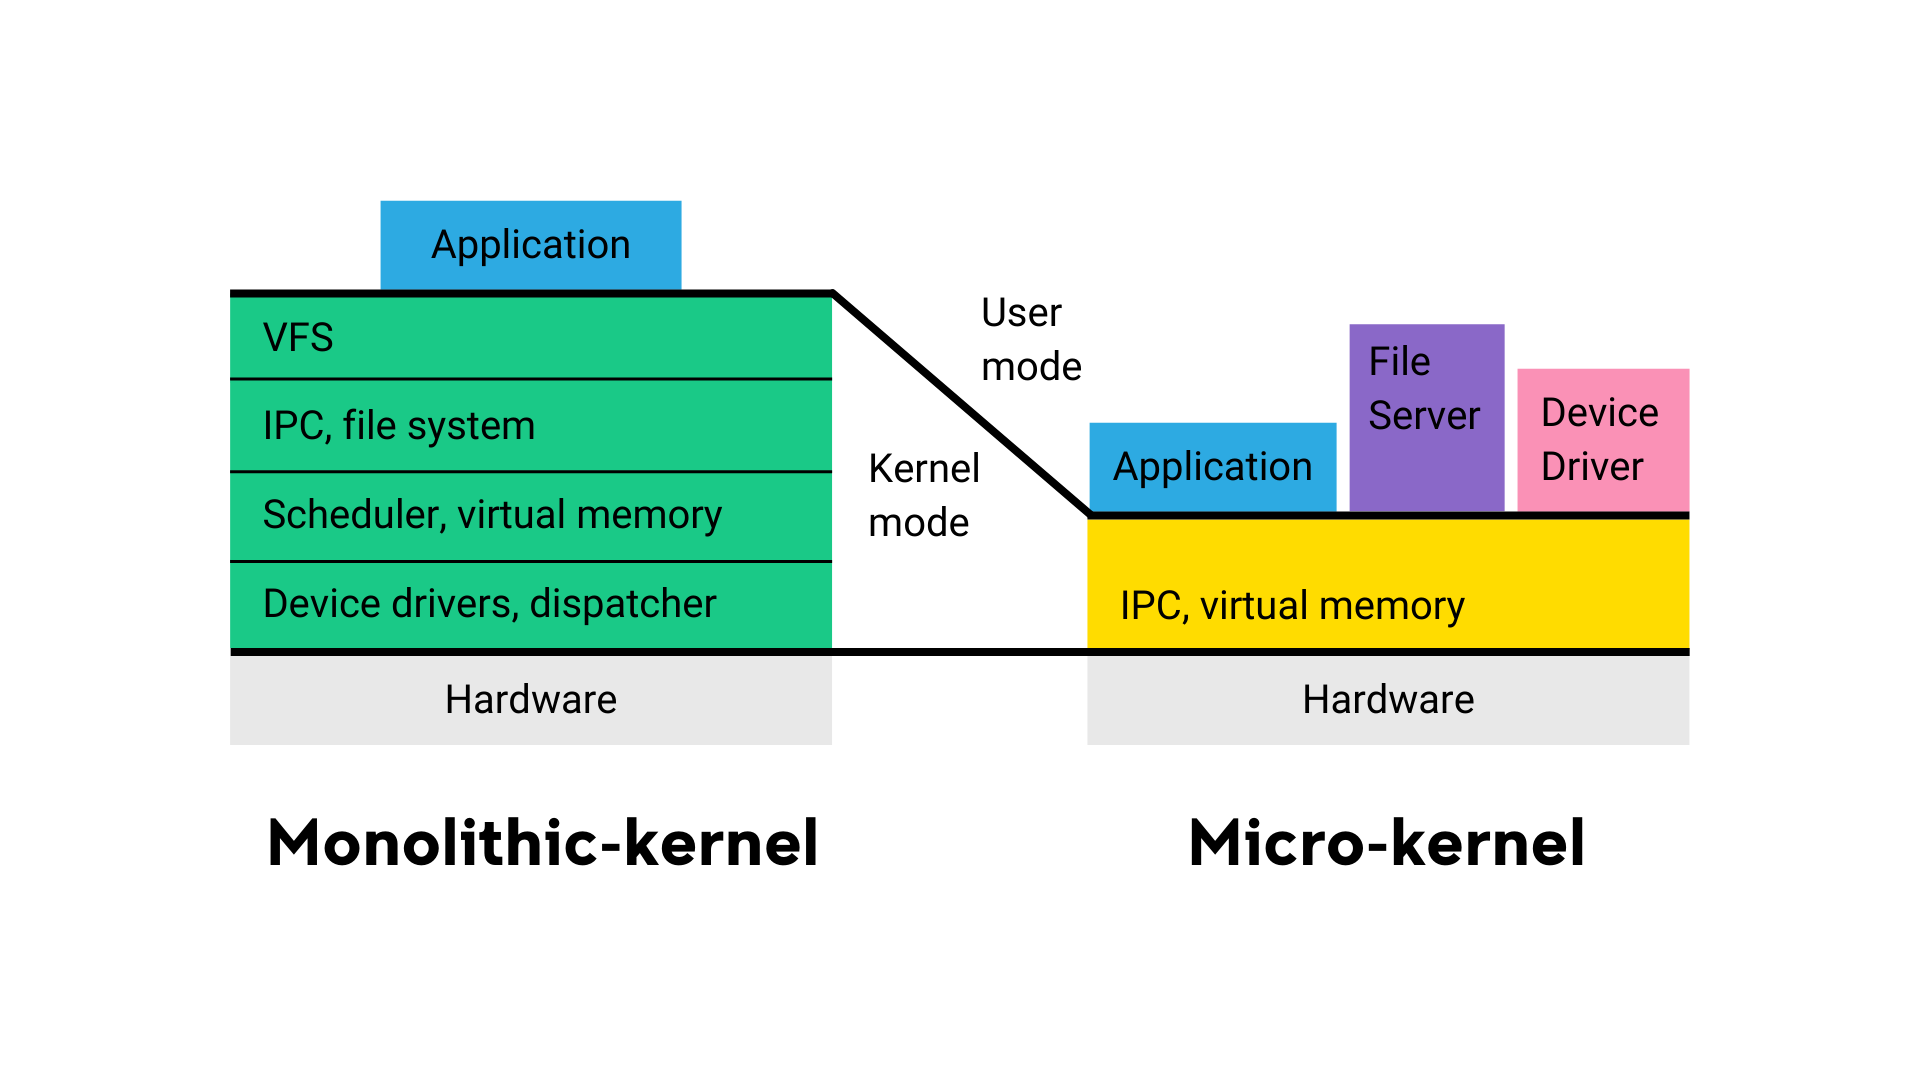
\includegraphics[width=\linewidth]{report-a_micro_v_mono}
    \caption{Comparison of monolithic and microkernels \cite{AOSMicrokernelSlide}.}
    \label{fig:sel4_microkernel}
\end{figure}

Since most system services do not reside in the kernel, but instead are implemented in user-space, it is critical that seL4 developers have sufficient tooling such that they can diagnose performance issues.